\chapter{La zone de localisation}

La zone de localisation permet � l'utilisateur de l'application de
savoir � chaque instant dans quel �tat se trouve l'application. Cette
zone est repr�sent� par des onglets (non cliquables).Par
exemple, si l'utilisateur est en train de consulter un exercice,
l'onglet se trouve sur {\it Compte}.\\
Cependant, cette zone contient plus ou moins de champs selon la nature
de l'utilisateur. En effet, un consultant ne pourra pas faire plus que
de consulter des projets ou TD.\\
Voici un aper�u des diff�rents �tats de la zone de localisation selon l'utilisateur.

\begin{flushleft}
\scalebox{0.6}{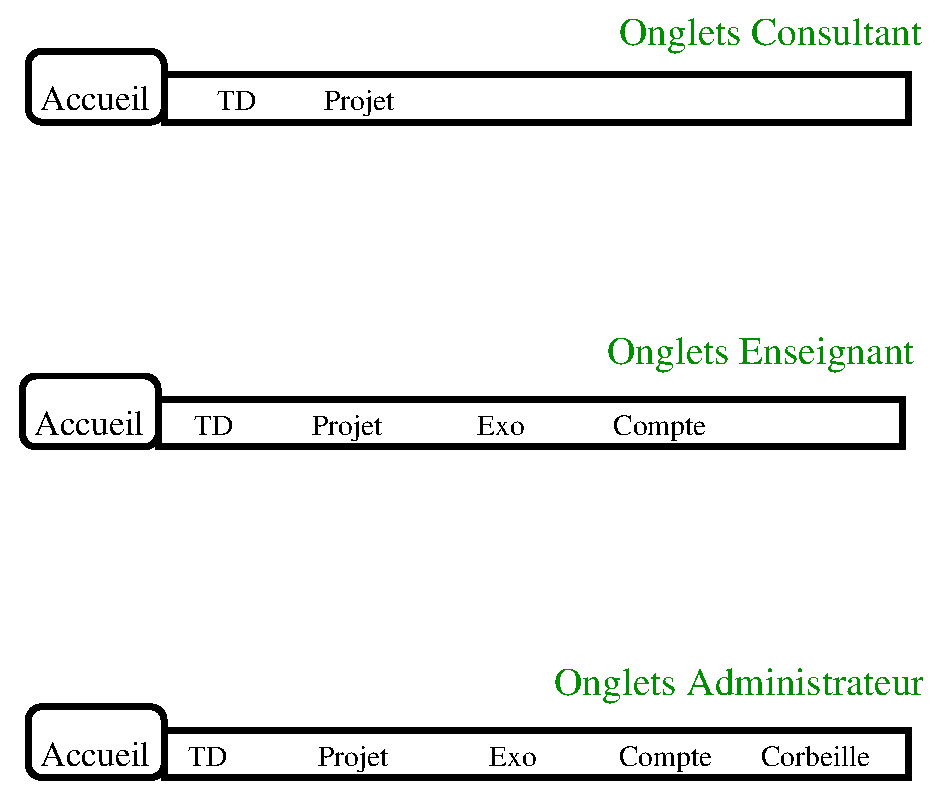
\includegraphics{../eps/onglets.eps}}\\
\end{flushleft}
